%%%%%%%%%%%%%%%%%%%% book.tex %%%%%%%%%%%%%%%%%%%%%%%%%%%%%
%
% sample root file for the chapters of your "monograph"
%
% Use this file as a template for your own input.
%
%%%%%%%%%%%%%%%% Springer-Verlag %%%%%%%%%%%%%%%%%%%%%%%%%%


% RECOMMENDED %%%%%%%%%%%%%%%%%%%%%%%%%%%%%%%%%%%%%%%%%%%%%%%%%%%
\documentclass[envcountsame,envcountchap]{tex/svmono}

% choose options for [] as required from the list
% in the Reference Guide, Sect. 2.2

\usepackage{makeidx}         % allows index generation
\usepackage{graphicx}        % standard LaTeX graphics tool
                             % when including figure files
\usepackage{multicol}        % used for the two-column index
\usepackage[bottom]{footmisc}% places footnotes at page bottom
% etc.
\usepackage{booktabs} % For formal tables
\usepackage[english]{babel}
\usepackage[utf8]{inputenc}
\usepackage{amsmath,amssymb}
\usepackage{graphicx}
\usepackage{array}
\usepackage[ruled,vlined,linesnumbered]{algorithm2e}
\usepackage{algorithmic}
\usepackage[colorinlistoftodos]{todonotes}
\usepackage{hyperref}
%\usepackage[mathscr]{eucal}
%\usepackage{MnSymbol}%
\usepackage{wasysym}%
\usepackage{booktabs} % multi column
\usepackage{listings}
\usepackage{multicol}
\setlength{\multicolsep}{0pt}
\usepackage{enumitem}


% see the list of further useful packages
% in the Reference Guide, Sects. 2.3, 3.1-3.3
\def\tt{{\sf true}}
\def\ff{{\sf false}}
\def\mltl{{\sf MLTL}\xspace}
\def\ltl{{\sf LTL}\xspace}
\def\U{{\mathcal{U}}}
\def\R{{\mathcal{R}}}

\makeindex             % used for the subject index
                       % please use the style svind.ist with
                       % your makeindex program


%%%%%%%%%%%%%%%%%%%%%%%%%%%%%%%%%%%%%%%%%%%%%%%%%%%%%%%%%%%%%%%%%%%%%

\begin{document}

\author{Iowa State University}
\title{R2U2 Developer Guide\\
{\small Work supported by NASA ECF NNX16AR57G and NSF CAREER Award CNS-1552934.}}
\subtitle{-- Monograph --}
\maketitle

\frontmatter%%%%%%%%%%%%%%%%%%%%%%%%%%%%%%%%%%%%%%%%%%%%%%%%%%%%%%


\tableofcontents


\mainmatter%%%%%%%%%%%%%%%%%%%%%%%%%%%%%%%%%%%%%%%%%%%%%%%%%%%%%%%
% %%%%%%%%%%%%%%%%%%%%%%%% part.tex %%%%%%%%%%%%%%%%%%%%%%%%%%%%%%%%%%
%
% sample part title
%
% Use this file as a template for your own input.
%
%%%%%%%%%%%%%%%%%%%%%%%% Springer-Verlag %%%%%%%%%%%%%%%%%%%%%%%%%%


\part{Part Title}

% %%%%%%%%%%%%%%%%%%%%% chapter.tex %%%%%%%%%%%%%%%%%%%%%%%%%%%%%%%%%
%
% sample chapter
%
% Use this file as a template for your own input.
%
%%%%%%%%%%%%%%%%%%%%%%%% Springer-Verlag %%%%%%%%%%%%%%%%%%%%%%%%%%

\chapter{Chapter Heading}
\label{intro} % Always give a unique label
% use \chaptermark{}
% to alter or adjust the chapter heading in the running head

Your text goes here. Separate text sections with the standard \LaTeX\
sectioning commands.

\section{Section Heading}
\label{sec:1}
% Always give a unique label
% and use \ref{<label>} for cross-references
% and \cite{<label>} for bibliographic references
% use \sectionmark{}
% to alter or adjust the section heading in the running head
Your text goes here. Use the \LaTeX\ automatism for your citations
\cite{monograph}.

\subsection{Subsection Heading}
\label{sec:2}
Your text goes here.

\begin{equation}
\vec{a}\times\vec{b}=\vec{c}
\end{equation}

\subsubsection{Subsubsection Heading}
Your text goes here. Use the \LaTeX\ automatism for cross-references as
well as for your citations, see Sect.~\ref{sec:1}.

\paragraph{Paragraph Heading} %
Your text goes here.

\subparagraph{Subparagraph Heading.} Your text goes here.%
%
\index{paragraph}
% Use the \index{} command to code your index words
%
% For tables use
%
\begin{table}
\centering
\caption{Please write your table caption here}
\label{tab:1}       % Give a unique label
%
% For LaTeX tables use
%
\begin{tabular}{lll}
\hline\noalign{\smallskip}
first & second & third  \\
\noalign{\smallskip}\hline\noalign{\smallskip}
number & number & number \\
number & number & number \\
\noalign{\smallskip}\hline
\end{tabular}
\end{table}
%
%
% For figures use
%
\begin{figure}
\centering
% Use the relevant command for your figure-insertion program
% to insert the figure file.
% For example, with the option graphics use
\includegraphics[height=4cm]{figure.eps}
%
% If not, use
%\picplace{5cm}{2cm} % Give the correct figure height and width in cm
%
\caption{Please write your figure caption here}
\label{fig:1}       % Give a unique label
\end{figure}
%
% For built-in environments use
%
\begin{theorem}
Theorem text goes here.
\end{theorem}
%
% or
%
\begin{lemma}
Lemma text goes here.
\end{lemma}
%
%
% Problems or Exercises should be sorted chapterwise
\section*{Problems}
\addcontentsline{toc}{section}{Problems}
%
% Use the following environment.
% Don't forget to label each problem;
% the label is needed for the solutions' environment
\begin{prob}
\label{prob1}
The problem\footnote{Footnote} is described here. The
problem is described here. The problem is described here.
\end{prob}

\begin{prob}
\label{prob2}
\textbf{Problem Heading}\\
(a) The first part of the problem is described here.\\
(b) The second part of the problem is described here.
\end{prob}



%

%\appendix
%\include{appendix}

\backmatter%%%%%%%%%%%%%%%%%%%%%%%%%%%%%%%%%%%%%%%%%%%%%%%%%%%%%%%
\chapter{Mission-Time Linear Temporal Logic}
\addcontentsline{toc}{chapter}{Future Time Runtime Verification}
\markboth{Mission-Time Linear Temporal Logic}{ft-RV}

\section{Definition of Future Time Runtime Verification}


\subsection{Mission-Time Linear Temporal Logic} Mission-Time Linear Temporal Logic (MLTL) \cite{r2u2} is future-time specification logic resembling Linear Temporal Logic, with finite integer bounds on the temporal operators.
An (closed) interval over naturals $I = [a, b]$ ($0\leq a\leq b$ are natural numbers) is a set of naturals
$\{i\ |\ a\leq i\leq b\}$.
%$I$ is \emph{bounded} iff $b < +\infty$, otherwise $I$ is \emph{unbounded}.
%\mltl involves only bounded intervals.
Unlike the Metric Temporal Logic (\textsf{MTL}) in \cite{AH94a}, it is not necessary to introduce open or half-open intervals over the natural domain; every open or half-open bounded interval corresponds to an equivalent closed bounded interval, e.g. (1,2) = $\emptyset$, (1,3) = [2,2], (1,3] = [2,3] and etc. Let $\mathcal{P}$ be a set of propositions, the syntax of a formula in Mission-time LTL (abbreviated as \mltl) is as follows.
\begin{center}
   	$\phi ::= \tt\ |\ \ff\ |\ p\ |\ \neg\phi\ |\ \phi\wedge\phi\ |\ \phi \U_I\phi\ |\ \phi \R_I\phi$;
\end{center}
%
where $I$ is a bounded interval, and $p\in\mathcal{P}$ is called an atom.
%We call $l$ is a \emph{literal} if $l$ is an atom or the negation of an atom.
The Until ($\U$) and Release ($\R$) are two temporal operators in \mltl.
Specially, we denote $F_I\phi$ to be $\tt$ $\U_I \phi$ (or $\Diamond_I \phi$) and $G_I\phi$ (or $\Box_I \phi$) to be $\ff$ $\mathcal{R}_I\phi$.
Notably, \mltl omits the Next (X) operator, which is essential in \ltl, due to the fact that
every Next formula $X\phi$ can be replaced by $G_{[1,1]}\phi$.

The semantics of \mltl formulas is interpreted over finite traces.
Let $\xi$ be a finite trace in which every point $\xi[i] (i\geq 0)$ is over $2^{\mathcal{P}}$, and $|\xi|$ denotes the length of
$\xi$ ($|\xi|<+\infty$ when
$\xi$ is a finite trace).
We use $\xi_i (i\geq 0)$ to represent the suffix of $\xi$ starting from position $i$ (including $i$). In particular, $\xi_i = \emptyset$ if $i\geq |\xi|$.
Now we define $\xi$ models (satisfies) an \mltl formula $\phi$, denoted as $\xi\models \phi$, as follows:

\begin{itemize}
	\item $\xi\models p$ iff $p\in\xi[0]$;
    \item $\xi\models \neg \phi$ iff $\xi\not\models\phi$;
    \item $\xi\models\phi_1\wedge\phi_2$ iff $\xi\models\phi_1$ and $\xi\models\phi_2$;
    \item $\xi\models \phi_1\U_I\phi_2$ iff there exists $i\in I$ such that, $\xi_i\models\phi_2$ and for every $j\in I$ s.t. $j<i$ it holds that $\xi_j\models\phi_1$;
    \item $\xi\models \phi_1\mathcal{R}_I\phi_2$ iff for every $i\in I$, either  $\xi_i\models\phi_2$ holds or there exists $j\in I$ and $j < i$ such that $\xi_j\models\phi_1$.
\end{itemize}

\subsection{From Gaped Results to Continued}
 %future time runtime verification basics
\chapter{Software Implementation of \mltl Verification}
\addcontentsline{toc}{chapter}{Software Implementation of \mltl Verification}
\markboth{Software Implementation of \mltl Verification}{SW-RV}

\section*{Dynamic Programming for \mltl Verification}


\subsubsection{Abstract Syntax Tree}
We use the dynamic programming proposed in [7] to compute the satisfaction of the MLTL. The first step is to break the MLTL formula into subformulas. We let the user describe their desired MLTL specification in a high-level (or assembly like) language. Then a compiler converts the formula into an Abstract Syntax Tree (AST). The AST explicitly exposes the logical connection between each observer node. We can then verify MLTL satisfaction of an input trace by checking the tree from leaf to root. For example, $\square_{[0,2]}(!a0)$ can be convert into the following execution sequence '$s0\rightarrow s1\rightarrow s2$' in our customized assembly language format:
\begin{equation*}
\begin{split}
 Line\, 0:\qquad & s0 \leftarrow load\: (a0,time)\\
 Line\, 1:\qquad & s1 \leftarrow \neg\: s0\\
 Line\, 2:\qquad & s2 \leftarrow \square_{[0,2]}\: s1
\end{split}
\end{equation*}

Where each subformula is an observer node (e.g., s0, s1, s2). The output from each node is a tuple containing a verdict and its corresponding timestamp (RTC) $\tau$. The last line $s2$ is the final result.

\subsubsection{Abstrct Syntax Tree (AST) Optimization}
For some \mltl formulas, certain sub-expressions occur more than once. An example formula is $G[2,4]a0\&!a0$. The compiler will generate an extra line of assembly code to load atomic $a0$ twice. Thus, it takes two separate queues for loading $a0$. There are two drawbacks of this: 1) memory resource wasting: extra queue is taken; 2) computation speed decrease: more assembly instructions to execute. Here we can do the following operations, as mentioned in~\cite{jakvsic2015signal}, to remove duplicate branches when synthesizing an \mltl formula into an AST. However, to support such optimization, the traditional hardware memory queue should be redesigned to support multiple readers. That is why we propose using an SCQ. The detailed optimization steps are described below. \par

\begin{figure}
\centering
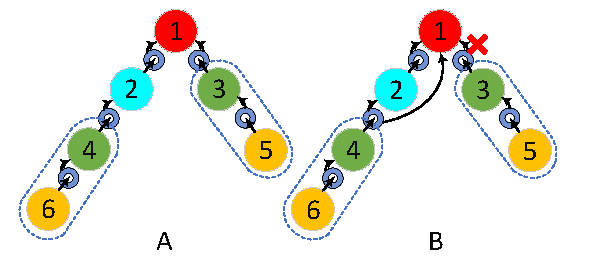
\includegraphics[width=0.65\textwidth]{fig/opt_ast.pdf}
\caption{\label{fig:ast}Example of optimizing an AST from A to B. Both node 3 and 4 share the same key string, so we cut edge (node 1 $\rightarrow$ node 3) and connect edge (node 1 $\rightarrow$ node 4). The connections of SCQs and nodes are also shown in the figure.}
\end{figure}

\begin{enumerate}
\item Do an inorder traverse to the unoptimized AST. Map each node to a string which represents its traverse order. We add '(' and ')' to each recursive traverse thus each string is uniquely represented in the branch structure.
\item Map each string to its root node. Whenever we traverse from a new node, we check whether the string already exists. If two strings are identical, we can reconnect the edge as shown in Figure.~\ref{fig:ast}.
\item Search from the root node to valid nodes in the tree. Then do a topological sort from the root node to arrange the node operator execution sequence.
\end{enumerate}


\subsubsection{Shared Connection Queue (SCQ)}
We employ what we call SCQs to store subformula results. An SCQ is a circular buffer (CB) with one write pointer and one or more read pointers. A similar data structure is proposed in \cite{4812537} for processing network streams. Figure.~\ref{fig:scq} shows how SCQs are embedded in an \mltl abstract syntax tree. There are two reasons we use the SCQ: 1) Each subformula may produce more than one tuple; 2) more than one parent nodes may read data from a given subformula.\par

The SCQ follows a writing rule called \textbf{Aggregation}, by which sequential input's timestamp will be overwritten by the later timestamp value if they have the same verdict. For example, if the data content is (true, 10), (false, 15), it means that during timestamp interval [11,15], the verdicts are all false. If the next input is (false, 16), the data content becomes (true, 10), (false, 16). The SCQ write and read algorithms are shown in Algorithm. \ref{ag:wr}, \ref{ag:rd}.\par
\begin{figure}
\centering
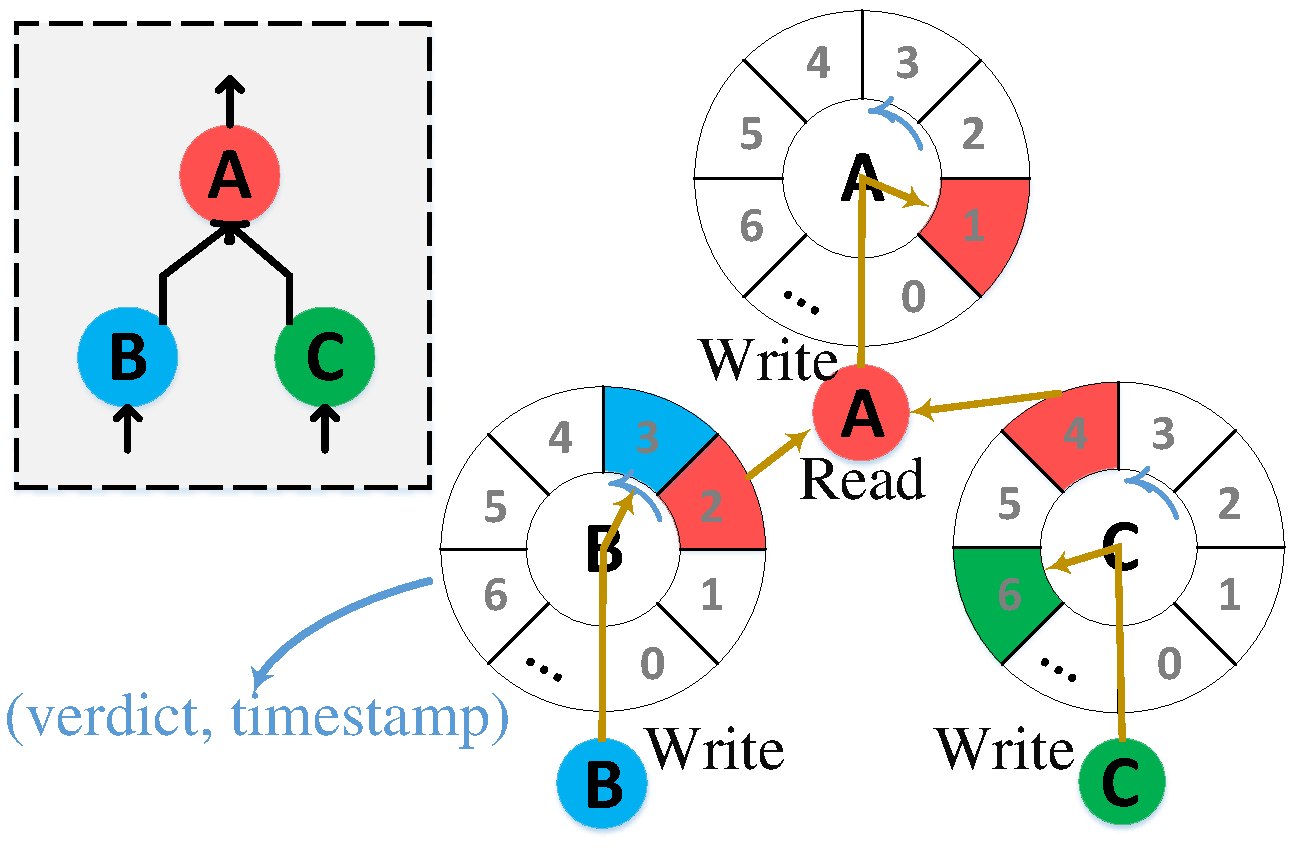
\includegraphics[width=0.6\textwidth]{fig/scq_cb.pdf}
\caption{\label{fig:scq}Detailed implementation of SCQs between observer nodes. The component in the dashed box is the abstract representation of connected observer nodes.}
\end{figure}





\section{Algorithm}
\subsection{SCQ Operation}

\subsubsection{Write}
The write operation algorithm is shown in Algorithm.~\ref{ag:wr}.

\begin{algorithm}
\SetAlgoLined
\SetKwInOut{Input}{input}
\Input{$new\_data$}
 \If{$new\_data$ is not Empty}{
 \If{$SCQ[SCQ.wr\_ptr].v == new\_data.v$}{$SCQ.wr\_ptr --$\;}
  $ SCQ[SCQ.wr\_ptr]\leftarrow new\_data$\;
  $SCQ.wr\_ptr ++$\;
  }
 \caption{\label{ag:wr}Function: write()}
\end{algorithm}

\subsubsection{Read}
The write operation algorithm is shown in Algorithm.~\ref{ag:rd}.
\begin{algorithm}
\SetAlgoLined
\SetKwInOut{Input}{input}
\SetKwInOut{Output}{output}
\Input{$\&rd\_ptr$, $\tau_e$}
\Output{$Empty$ or $read\_data$}
  \If{read}{
  \If{$*rd\_ptr==SCQ.wr\_ptr$}{
    \KwRet{Empty}\;
  }
    $read\_data\leftarrow SCQ[*rd\_ptr]$\;
    \While{$read\_data.\tau <\tau_e$}{
      $rd\_ptr++$\;
      \If{$*rd\_ptr==SCQ.wr\_ptr$}{
        \KwRet{Empty}\;
      }
      $read\_data\leftarrow SCQ[*rd\_ptr]$\;
    }
   \KwRet{$read\_data$}\;
  }
 \caption{\label{ag:rd}Function: read()}
\end{algorithm}

\subsection{Temporal Operator}
\subsubsection{Load}
The Load operator algorithm is shown in Algorithm.~\ref{ag:at}.
\begin{algorithm}
\SetAlgoLined
\SetKwInOut{Input}{input}
\SetKwInOut{Output}{output}
\Input{$atomic$, $current\_time$, SCQ for write ($SCQ\_wr$)}
\If{write}{
$SCQ\_wr.write([current\_time,atomic]$)\;
}
 \caption{\label{ag:at}LOAD Operation}
\end{algorithm}

\subsubsection{Negate Operation}
The Negate operator algorithm is shown in Algorithm.~\ref{ag:ne}.
\begin{algorithm}
\SetAlgoLined
\SetKwInput{KwData}{Var}
\SetKwInOut{Input}{input}
\SetKwInOut{Output}{output}
\KwData{$\tau_e$}
\Input{SCQ for read ($SCQ\_rd$), SCQ for write ($SCQ\_wr$)}
\While{$SCQ\_rd$ is \textbf{not} Empty}{
  $read\_data \leftarrow SCQ\_rd.read(\tau_e,\&rd\_ptr)$\;
  $SCQ\_wr.write(!read\_data.\tau,read\_data.v)$\;
  $\tau_e \leftarrow read\_data.\tau+1$\;
}
 \caption{\label{ag:ne}NEGATION Operator: $\neg$}
\end{algorithm}

\subsubsection{Global Operation}
Formula $\square_{[lb,ub]} a0$ defines the behavior of the atomic propositions $a0$ during a future time interval, which is specified by a lower bound ($lb$) and an upper bound ($ub$). The algorithm is shown in Algorithm.~\ref{ag:gl}. First, the algorim loads data from $SCQ\_rd$ following Algorithm.~\ref{ag:rd}. We use $m_\uparrow$ to record the rising edge (i.e., \textbf{false} to \textbf{true} verdict transition) of the $a0$. When the rising edge occurs, we start counting the length of consecutive \textbf{true} verdicts of $a0$, since $a0$ should remain \textbf{true} during $[lb,ub]$. If $a0$ turns \textbf{false} at a certain RTC, the algorithm will return the tuple $(false, RTC-lb)$. If $a0$ remains true over the interval $[lb,ub]$, it will return $(true, RTC-ub)$. The algorithm will continue looping as long as the $SCQ\_rd$ is nonempty.
\begin{algorithm}
\SetAlgoLined
\SetKwInput{KwData}{Var}
\SetKwInOut{Input}{input}
\SetKwInOut{Output}{output}
\SetKwComment{comment}{$\LHD$}{}
\SetKwInput{KwInit}{Init}
\KwData{$m_\uparrow$, $(\tau_{pre},v_{pre})$, $\tau_e$}
\KwInit{$(\tau_{pre},v_{pre}) \leftarrow (-1,\ff)$}
\Input{SCQ for read ($SCQ\_rd$), SCQ for write ($SCQ\_wr$)}
$data = SCQ\_rd.read(\tau_e,\&rd\_ptr)$\;
\While{$data$ is \textbf{not} Empty}{
 $\tau_e = data.\tau +1$\;
 % \If{$data.v$ \textbf{and} $!v_{pre}$}{ %
 \If{$data.v$ \textbf{and} $!v_{pre}$}{% can init as (0,\ff)
    $m_\uparrow \leftarrow \tau_{pre} + 1$\;
 }
 \uIf{$data.v$}{
  \If{$data.\tau -m_\uparrow \geq ub-lb$ \textbf{and} $data.\tau - ub \geq 0$}{
      $SCQ\_wr.write([data.\tau - ub, \tt])$\;
  }}
  \ElseIf{$data.\tau -lb \geq 0$}{
      $SCQ\_wr.write([data.\tau - lb, \ff])$\;
  }
  $(\tau_{pre},v_{pre}) \leftarrow data$\;
  $data = SCQ\_rd.read(\tau_e,\&rd\_ptr)$\;
}
 \caption{\label{ag:gl}GLOBAL Operation: $\square_{[lb,ub]}$}
\end{algorithm}

\subsubsection{Future Operator}
The Future operator algorithm is shown in Algorithm.~\ref{ag:fu}.
\begin{algorithm}
\SetAlgoLined
\SetKwInput{KwData}{Var}
\SetKwInput{KwInit}{Init}
\SetKwInOut{Input}{input}
\SetKwInOut{Output}{output}
\KwData{$m_\downarrow$, $(\tau_{pre},v_{pre})$, $\tau_e$}
\KwInit{$(\tau_{pre},v_{pre}) \leftarrow (0,\ff)$ or $(\tau_{pre},v_{pre}) \leftarrow (-1,\tt)$ }
\Input{SCQ for read ($SCQ\_rd$), SCQ for write ($SCQ\_wr$)}
$data = SCQ\_rd.read(\tau_e,\&rd\_ptr)$\;
\While{$data$ is \textbf{not} Empty}{
 $\tau_e = data.\tau +1$\;
 \If{$!data.v$ \textbf{and} $v_{pre}$}{
    $m_\downarrow \leftarrow \tau_{pre} + 1$\;
 }
 \uIf{$!data.v$}{
  \If{$data.\tau -m_\downarrow \geq ub-lb$ \textbf{and} $data.\tau - ub \geq 0$}{
      $SCQ\_wr.write([data.\tau - ub, \ff])$\;
  }}
  \ElseIf{$data.\tau -lb \geq 0$}{
      $SCQ\_wr.write([data.\tau - lb, \tt])$\;
  }
  $(\tau_{pre},v_{pre}) \leftarrow data$\;
  $data = SCQ\_rd.read(\tau_e,\&rd\_ptr)$\;
}
 \caption{\label{ag:fu}FUTURE Operation: $\Diamond_{[lb,ub]}$}
\end{algorithm}

\subsubsection{And Operation}
The AND algorithm reads data from two SCQs. If any of the data tells false and that timestamp $\tau$ is larger, the operator can immediately return $(\ff,\tau)$. The AND operator requires both inputs' verdicts are true to returns true requires, and chooses the smaller timestamp.
\begin{algorithm}
\SetAlgoLined
\SetKwInput{KwData}{Var}
\SetKwInOut{Input}{input}
\SetKwInOut{Output}{output}
\KwData{$\tau_e$}
\Input{Left SCQ for read ($SCQ\_1\_rd$), Right SCQ for read ($SCQ\_2\_rd$), SCQ for write ($SCQ\_wr$)}
$result \leftarrow [-1,\ff]$\;
$data\_1 \leftarrow SCQ\_1\_rd.read(\tau_e,\&rd\_ptr)$\;
$data\_2 \leftarrow SCQ\_2\_rd.read(\tau_e,\&rd\_ptr)$\;
\While{$data\_1$ is \textbf{not} Empty $||$ $data\_2$ is \textbf{not} Empty}{
  \uIf{both $data\_1$ \textbf{and} $data\_2$ are \textbf{not} empty}{
    \uIf{$data\_1.v$ \textbf{and} $data\_2.v$}{$result = [min(data\_1.\tau,data\_2.\tau),\tt]$\;}
    \uElseIf{$!data\_1.v$ \textbf{and} $!data\_2.v$}{$result = [max(data\_1.\tau,data\_2.\tau),\ff]$\;}
    \uElseIf{$data\_1.v$}{$result = [data\_2.\tau,\ff]$\;}
    \Else{$result = [data\_1.\tau,\ff]$\;}
  }
  \uElseIf{$data\_1$ is Empty}{
    \If{$!data\_2.v$}{$result = [data\_2.\tau,\ff]$\;}
  }\ElseIf{$!data\_1.v$}{
    $result = [data\_1.\tau,\ff]$\;}
  \uIf{$result.\tau != -1$}{
    $SCQ\_wr.write(result)$\;
    $\tau_e \leftarrow result.\tau+1$\;
  }\Else{Break\;}
  $data\_1 \leftarrow SCQ\_1\_rd.read(\tau_e,\&rd\_ptr)$\;
  $data\_2 \leftarrow SCQ\_2\_rd.read(\tau_e,\&rd\_ptr)$\;
}
 \caption{\label{ag:and}AND Operation: $\wedge$}
\end{algorithm}

\subsubsection{Or Operation}
The Or operator algorithm is shown in Algorithm.~\ref{ag:or}.
\begin{algorithm}
\SetAlgoLined
\SetKwInput{KwData}{Var}
\SetKwInOut{Input}{input}
\SetKwInOut{Output}{output}
\KwData{$\tau_e$}\
\Input{Left SCQ for read ($SCQ\_1\_rd$), Right SCQ for read ($SCQ\_2\_rd$), SCQ for write ($SCQ\_wr$)}
$result \leftarrow [-1,\ff]$\;
$data\_1 \leftarrow SCQ\_1\_rd.read(\tau_e,\&rd\_ptr)$\;
$data\_2 \leftarrow SCQ\_2\_rd.read(\tau_e,\&rd\_ptr)$\;
\While{$data\_1$ is \textbf{not} Empty $||$ $data\_2$ is \textbf{not} Empty}{
  \uIf{both $data\_1$ \textbf{and} $data\_2$ are \textbf{not} empty}{
    \uIf{$data\_1.v$ \textbf{or} $data\_2.v$}{$result = [max(data\_1.\tau,data\_2.\tau),\tt]$\;}
    \uElseIf{$!data\_1.v$ \textbf{and} $!data\_2.v$}{$result = [min(data\_1.\tau,data\_2.\tau),\ff]$\;}
    \uElseIf{$data\_1.v$}{$result = [data\_1.\tau,\tt]$\;}
    \Else{$result = [data\_2.\tau,\tt]$\;}
  }
  \uElseIf{$data\_1$ is Empty}{
    \If{$data\_2.v$}{$result = [data\_2.\tau,\tt]$\;}
  }\ElseIf{$data\_1.v$}{$result = [data\_1.\tau,\tt]$\;}
  \uIf{$result.\tau != -1$}{
    $SCQ\_wr.write(result)$\;
    $\tau_e \leftarrow result.\tau+1$\;
  }\Else{Break\;}
  $data\_1 \leftarrow SCQ\_1\_rd.read(\tau_e,\&rd\_ptr)$\;
  $data\_2 \leftarrow SCQ\_2\_rd.read(\tau_e,\&rd\_ptr)$\;
}
 \caption{\label{ag:or}OR Operation: $\vee$}
\end{algorithm}

\subsubsection{Until Operation}
The Until operator algorithm is shown in Algorithm.~\ref{ag:un}.
\begin{algorithm}
\SetAlgoLined
\SetKwInput{KwData}{Var}
\SetKwInput{KwInit}{Init}
\SetKwComment{comment}{$\LHD$}{}
\SetKwInOut{Input}{input}
\SetKwInOut{Output}{output}
\KwData{$m_\downarrow$, $(\tau_{pre},v_{pre})$, $\tau_e$, $\tau_{res}$}
\KwInit{$(\tau_{pre},v_{pre}) \leftarrow (0,\ff)$ or $(\tau_{pre},v_{pre}) \leftarrow (-1,\tt)$, $\tau_{res}\leftarrow 0$}
\Input{Left SCQ for read ($SCQ\_1\_rd$), Right SCQ for read ($SCQ\_2\_rd$), SCQ for write ($SCQ\_wr$)}
$data\_1 = SCQ\_1\_rd.read(\tau_e,\&rd\_ptr)$\;
$data\_2 = SCQ\_2\_rd.read(\tau_e,\&rd\_ptr)$\;
\While{$data\_1$ is \textbf{not} Empty \textbf{and} $data\_2$ is \textbf{not} Empty}{
  $result =[-1,\ff]$\;
 $t_{min} = min(data\_1.\tau ,data\_2.\tau )$\;
 $\tau_e \leftarrow t_{min}+1$\;
 \If{$v_{pre}$ \textbf{and} $!data\_2.v$}{
    % $m_\downarrow \leftarrow t_{min}$\;
    $m_\downarrow \leftarrow \tau_{pre}+1$\;
 }
 \uIf{$data\_2.v$}{
    $result \leftarrow [t_{min}-lb,\tt]$\;
 }\uElseIf{$!data\_1.v$}{
    $result \leftarrow [t_{min}-lb,\ff]$\;
 }\ElseIf{$t_{min}\geq ub-lb+m_\downarrow$}{
    $result \leftarrow [t_{min}-ub,\ff]$%\comment*[r]{for strong until $\mathcal{U}$}
    % \tcc*[r]{$\LHD$ for $\mathcal{U}$}
    % $result \leftarrow [t_{min}-ub,\tt]$%\comment*[r]{for weak until $\mathcal{W}$}
 }
 \If{$result.\tau \geq \tau_{res}$}{
     $\tau_{res}\leftarrow result.\tau + 1$\;
     $SCQ\_wr.write(result)$\;
 }
$(\tau_{pre},v_{pre}) \leftarrow data\_2$\;
$data\_1 = SCQ\_1\_rd.read(\tau_e,\&rd\_ptr)$\;
$data\_2 = SCQ\_2\_rd.read(\tau_e,\&rd\_ptr)$\;
}

 \caption{\label{ag:un}UNTIL Operation: $\mathcal{U}_{[lb,ub]}$}
\end{algorithm}




\subsection{SCQ Utilization}
Most of the observer processor core's memory is used by the input SCQs for binary operators: $\wedge$, $\vee$ and $\mathcal{U}$. Due to the timestamp mismatch between the two inputs, the input with a more recent timestamp has to be stalled in the SCQ. Here we define the best-case-delay (\textbf{bcd}) and worst-case-delay (\textbf{wcd}) to analyse the timestamp mismatch. The \textbf{bcd} is the earliest or best delay output time relative to the current real-time clock (RTC) and \textbf{wcd} in the latest/worst delay. The delay is produced by temporal operators like $\square$, $\Diamond$ and $\mathcal{U}$. Each temporal operator adds the $lb$ to \textbf{bcd} and $ub$ to \textbf{wcd}. The maximum size of a given SCQ can be determined by taking its \textbf{bcd} and minus the \textbf{wcd} of the other input.\par

To allocate the SCQ size for all operator nodes, we first recursively decide the \textbf{bcd} and \textbf{wcd} of each operator from the bottom to the root node. Algorithm.~\ref{ag:sq} then uses this information to compute the queue size for each node.\par


\begin{algorithm}
    \SetAlgoLined
    \SetKwInput{KwData}{Var}
    \SetKwInOut{KwInit}{Init}
    \SetKwProg{Fn}{Function}{}{end}
    \SetKwComment{comment}{$\LHD$}{}
    % \SetKwInOut{Input}{input}
    % \SetKwInOut{Output}{output}
    % \KwData{$\tau_e$}\
    % \Input{ss}\
    
    \KwInit{assign all nodes' output SCQ size $\leftarrow$ 1}
    compute \textbf{bcd} and \textbf{wcd} of each node from bottom up\;
    \For{every node $\mathcal{N}$}{
      assign output SCQ size of $\mathcal{N}$\;
    }
    
    
    \Fn{assign output SCQ size (node $\mathcal{N}$)}{
    set $\{wcd\} \leftarrow \varnothing$ \;
    \For{$\mathcal{N}$'s every binary parent node $\mathcal{N}.bp$}{
      add \textbf{wcd} of the other child node of $\mathcal{N}.bp$ to $\{wcd\}$\;
    }
    find the maximum \textbf{wcd} of $\{wcd\}$ set: $max(wcd)$\;
    get output SCQ size of $\mathcal{N} \leftarrow max(wcd)-\mathcal{N}.bcd+1$\;
    }
     \caption{\label{ag:sq}Determine the size of SCQ}
\end{algorithm}


Detailed implementation of Algorithm. \ref{ag:sq}.
\begin{algorithm}
\SetAlgoLined
\SetKwInput{KwData}{Var}
\SetKwProg{KwInit}{Init}{}{end}
\SetKwProg{Fn}{Function}{}{end}
\SetKwComment{comment}{$\LHD$}{}
% \SetKwInOut{Input}{input}
% \SetKwInOut{Output}{output}
% \KwData{$\tau_e$}\
% \Input{ss}\

\KwInit{}{
\For{all node n in observer node set}{
  Init $n.SCQ\_size \leftarrow 1$
  \If{$n.operator = \mathcal{L}$}{
    $n.bcd, n.wcd \leftarrow 0, 0$\;
    put node $n$ in $visited[]$\;
  }
}
}
$Assign\_Queue\_Size($root node$)$\;
\Fn{Assign\_Queue\_Size(node n)}{
  \If{n.operator == $\wedge | \vee | \mathcal{U}$}{
    $\mu \leftarrow n.left\_child$\;
    $\nu \leftarrow n.right\_child$\;
    \If{$\mu$ \textbf{not} in $visited[]$}{
      $Assign\_Queue\_Size(\mu)$\;
    }
    \If{$\nu$ \textbf{not} in $visited[]$}{
      $Assign\_Queue\_Size(\nu)$\;
    }
    \uIf{n.operator == $\wedge | \vee$}{
      $n.bcd \leftarrow min(\mu.bcd, \nu.bcd)$\;
      $n.wcd \leftarrow max(\mu.wcd, \nu.wcd)$\;
    }\ElseIf{n.operator == $\mathcal{U}$}{
      $n.bcd \leftarrow min(\mu.bcd, \nu.bcd) + min(n.J)$\;
      $n.wcd \leftarrow max(\mu.wcd, \nu.wcd) + max(n.J)$\;
    }
	   $\mu.SCQ\_size\leftarrow max(\mu.SCQ\_size,\nu.wcd-\mu.bcd+1)$\;
	   $\nu.SCQ\_size\leftarrow max(\nu.SCQ\_size,\mu.wcd-\nu.bcd+1)$\;
  }
  \If{n.operator == $\square | \Diamond | \neg$}{
    $\mu \leftarrow n.child$\;
    \If{$\mu$ \textbf{not} in $visited[]$}{
      $Assign\_Queue\_Size(\mu)$\;
    }
    \uIf{n.operator == $\square | \Diamond$}{
      $n.bcd \leftarrow \mu.bcd + min(n.J)$\;
      $n.wcd \leftarrow \mu.wcd + max(n.J)$\;
    }\ElseIf{n.operator == $\neg$}{
      $n.bcd \leftarrow \mu.bcd$\;
      $n.wcd \leftarrow \mu.wcd$\;
    }
  }
  put node $n$ in $visited[]$\;
}
 \caption{\label{ag:sq_d}Determine the size of SCQ}
\end{algorithm}




\section*{\mltl Grammar Definition}
A compiler implementation for parsing \mltl formula is written in python. The compiler is divided into two parts: \textbf{Lexer}(ply.lex) and \textbf{Parser}(ply.yacc). 
\begin{lstlisting}[language=Python,basicstyle=\small]
'''
expression 	: expression AND expression
            | expression OR expression
            | NEG expression
            | GLOBAL LBRACK NUMBER RBRACK expression
            | GLOBAL LBRACK NUMBER COMMA NUMBER RBRACK expression
            | FUTURE LBRACK NUMBER RBRACK expression
            | FUTURE LBRACK NUMBER COMMA NUMBER RBRACK expression
            | expression UNTIL LBRACK NUMBER RBRACK expression
            | expression UNTIL LBRACK NUMBER COMMA NUMBER RBRACK expression
            | expression WEAK_UNTIL LBRACK NUMBER RBRACK expression
            | expression WEAK_UNTIL LBRACK NUMBER COMMA NUMBER RBRACK expression			
'''
precedence = (
    ('left', 'AND', 'OR'),
    ('left', 'GLOBAL', 'FUTURE', 'UNTIL','WEAK_UNTIL'),	
    ('left', 'NEG'),
    ('left', 'LPAREN', 'RPAREN','ATOMIC','LBRACK','RBRACK'),
)
\end{lstlisting}
\chapter{\mltl Runtime Verification on Hardware}
\addcontentsline{toc}{chapter}{\mltl Runtime Verification on Hardware}
\markboth{HW-RV}{HW-RV}

\section{Future Time MLTL Processor Architecture}

The \mltl observer core handles processing the assembly code with sensor data as input. The observer core can execute eight \mltl operations, namely LOAD ($\mathcal{L}$), NEGATION ($\neg$), GLOBAL ($\square$), FUTURE ($\Diamond$), AND ($\wedge$), OR ($\vee$) and UNTIL ($\U$). The system is responsible for the following tasks:
\begin{enumerate}
  \item Filtering the digital sensor signals and converting the signals into atomic propositions (APs);
  \item Using the Load command ($\mathcal{L}$) to load APs into SCQs;
  \item Executing assembly line by line and returning the final result.
\end{enumerate}

Figure.~\ref{fig:wf} shows the finite state machine inside the processing core. Each operator except $\mathcal{L}$, keeps looping until the source SCQ is empty. Thus, each instruction can potentially write back more than one results to current SCQ. Next, the programme counter (PC) increases and next instruction is fetched. During each real time clock (RTC) tick or sampling period, the core completes executing all commands in the instruction BRAM. Operators like $\square$, $\Diamond$ and $\mathcal{U}$ introduce local variables in the algorithm. In the hardware, we also use BRAMs to store these local variables and pointers.\\
\begin{figure}
\centering
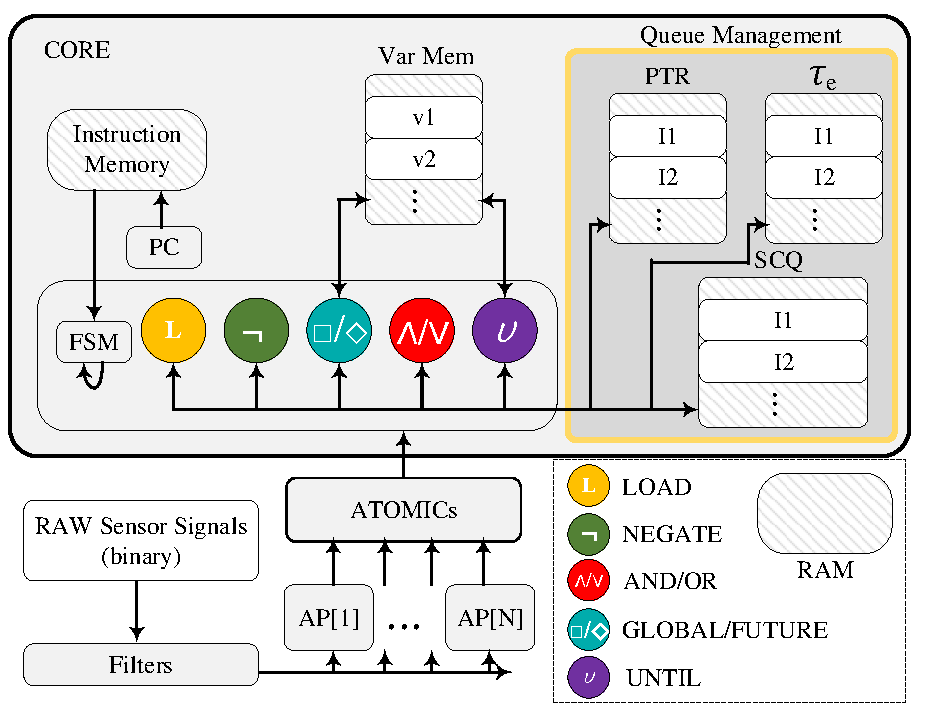
\includegraphics[width=0.55\textwidth]{fig/core.pdf}
\caption{\label{fig:core}Computation core of the observer.}
\end{figure}

\begin{figure}
\centering
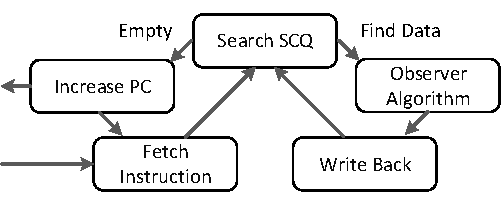
\includegraphics[width=0.55\textwidth]{fig/wf.pdf}
\caption{\label{fig:wf}State machine transitions of the observer processing core.}
\end{figure}


\section*{Interface for Configuring Hardware Monitor}
We use UART to communicate between FPGA and PC. The PC is used as the 


\section*{Case Study}
\subsection{Verfication on R2}



\bibliographystyle{abbrv}
\bibliography{referenc}
\printindex

%%%%%%%%%%%%%%%%%%%%%%%%%%%%%%%%%%%%%%%%%%%%%%%%%%%%%%%%%%%%%%%%%%%%%%

\end{document}





